\chapter{Summary}\label{c:summary}

\section{Speed comparison}\label{summary:speed}

\definecolor{bblue}{HTML}{4F81BD}
\definecolor{rred}{HTML}{C0504D}
\definecolor{ggreen}{HTML}{9BBB59}

In this section we show the results of performance benchmarks.

\subsection{Single-threaded benchmarks}

First, we compared the performance of the reference program, the new program running in the legacy mode, which replicates the behavior of the reference version exactly, and the new program running in the release mode, which uses the new optimizations. We performed three benchmarks, for three values of the number of pseudoatoms. Figure \ref{f:bench_single} shows the normalized results of the benchmarks. As we can see, the performance of the new implementation is comparable with the performance of the Fortran version. In particular, the abstractions and the introduced quality-of-life improvements did not affect its speed considerably. At the same time, newly-introduced optimizations make it even faster.

\begin{figure}[ht]
\centering
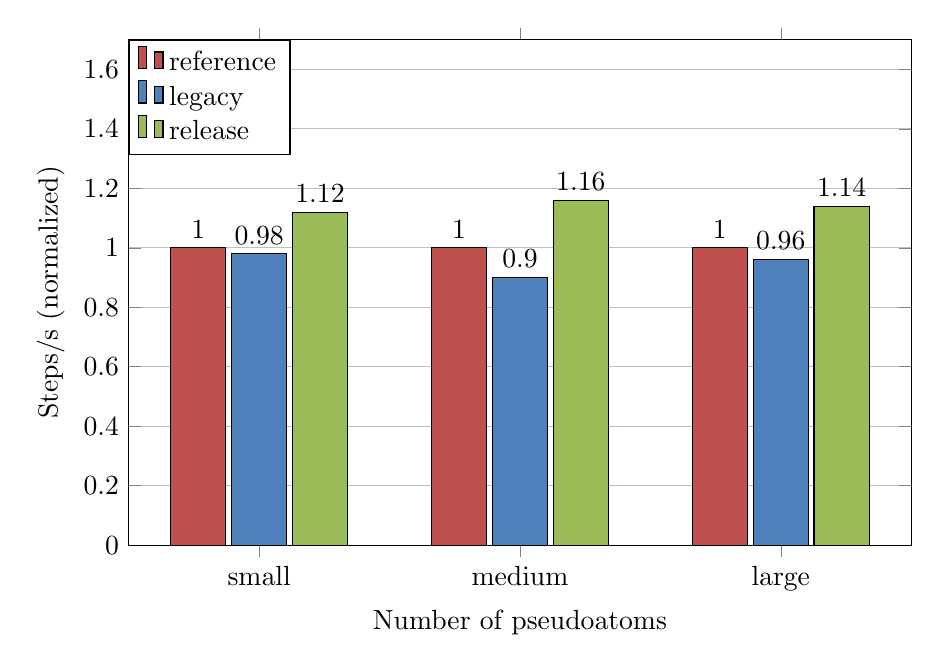
\begin{tikzpicture}
\begin{axis}[
        width  = 0.95*\textwidth,
        height=8cm,
        ybar,
        bar width=20pt,
        ymajorgrids = true,
        symbolic x coords={small,medium,large},
        xtick = data,
        enlarge x limits=0.25,
        nodes near coords,
        ymin=0,
        ymax=1.7,
        legend style={
                at={(0,1)},
                anchor=north west
        },
        legend cell align=left,
        ylabel = {Steps/s (normalized)},
        xlabel = {Number of pseudoatoms}
    ]
\addplot [style={black,fill=rred,mark=none}]
	coordinates {(small,1.00) (medium,1.00) (large,1.00)};
\addplot [style={black,fill=bblue,mark=none}]
	coordinates {(small,0.98) (medium,0.90) (large,0.96)};
\addplot [style={black,fill=ggreen,mark=none}]
	coordinates {(small,1.12) (medium,1.16) (large,1.14)};
\legend{reference, legacy, release}
\end{axis}
\end{tikzpicture}
\caption{Single-threaded benchmarks}
\label{f:bench_single}
\end{figure}

\subsection{Multi-threaded benchmark}

Next, we compared the performance of the three aforementioned versions in a multi-threaded context. Figure \ref{f:bench_multi} shows the normalized results of the ``large'' benchmark. As we can see, the reference implementation benefited from the use of additional cores only by around 55\%, having stalled out at around 4 threads. Our implementation exhibits more favorable behavior, reaching a speedup 160\% higher than the Fortran version when using 8 threads. Combined with the fact that our implementation is slightly faster in the single-threaded setting, this shows that the new program is 193\% faster on this benchmark.

\begin{figure}[ht]
\centering
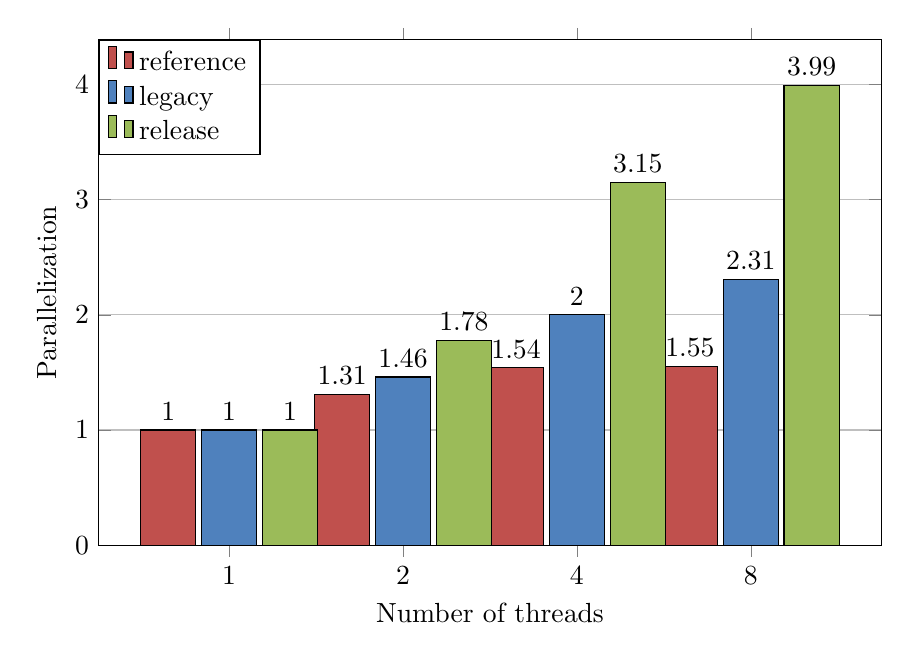
\begin{tikzpicture}
\begin{axis}[
        width  = 0.95*\textwidth,
        height=8cm,
        ybar,
        bar width=20pt,
        ymajorgrids = true,
        symbolic x coords={1,2,4,8},
        xtick = data,
        enlarge x limits=0.25,
        nodes near coords,
        ymin=0,
        legend style={
                at={(0,1)},
                anchor=north west
        },
        legend cell align=left,
        ylabel = {Parallelization},
        xlabel = {Number of threads}
    ]
\addplot [style={black,fill=rred,mark=none}]
	coordinates {(1,1.00) (2,1.31) (4,1.54) (8,1.55)};
\addplot [style={black,fill=bblue,mark=none}]
	coordinates {(1,1.00) (2,1.46) (4,2.00) (8,2.31)};
\addplot [style={black,fill=ggreen,mark=none}]
	coordinates {(1,1.00) (2,1.78) (4,3.15) (8,3.99)};
\legend{reference, legacy, release}
\end{axis}
\end{tikzpicture}

\caption{Multi-threaded benchmarks}
\label{f:bench_multi}
\end{figure}

\section{Publication}

The new program is to be published together with a revised version of the paper submitted to \textit{Computer Physics Communications} \cite{CPC14}. At the moment, we are working on the revision together with the researchers at the Institute of Physics of the Polish Academy of Sciences. They expect that the new program will fully replace the old one.